\documentclass[12pt]{article}
\usepackage{amsthm,amssymb,amsmath,amsfonts}
\usepackage[a4paper, top=25mm, bottom=30mm, left=25mm, right=25mm]{geometry}
\usepackage[pagebackref=false,colorlinks,linkcolor=black,citecolor=black]{hyperref}
\usepackage[nameinlink]{cleveref}
 \AtBeginDocument{%
    \crefname{equation}{برابری}{equations}%
    \crefname{chapter}{فصل}{chapters}%
    \crefname{section}{بخش}{sections}%
    \crefname{appendix}{پیوست}{appendices}%
    \crefname{enumi}{مورد}{items}%
    \crefname{footnote}{زیرنویس}{footnotes}%
    \crefname{figure}{شکل}{figures}%
    \crefname{table}{جدول}{tables}%
    \crefname{theorem}{قضیه}{theorems}%
    \crefname{lemma}{لم}{lemmas}%
    \crefname{corollary}{نتیجه}{corollaries}%
    \crefname{proposition}{گزاره}{propositions}%
    \crefname{definition}{تعریف}{definitions}%
    \crefname{result}{نتیجه}{results}%
    \crefname{example}{مثال}{examples}%
    \crefname{remark}{نکته}{remarks}%
    \crefname{note}{یادداشت}{notes}%
    \crefname{observation}{مشاهده}{observations}%
    \crefname{algorithm}{الگوریتم}{algorithms}%
    \crefname{cproof}{برهان}{cproofs}%
}

\usepackage{tikz}
\usepackage{graphicx}
\usepackage{booktabs}
\usepackage{color}
\usepackage{graphicx}
\usepackage{subcaption}

\usepackage{setspace}
\doublespacing

\usepackage{titletoc}
\usepackage{tocloft}
\usepackage{enumitem}
\usepackage{amsmath, amssymb}
\usepackage{algorithm}
\usepackage[noend]{algorithmic}
\renewcommand{\algorithmicrequire}{\textbf{Input:}}
\renewcommand{\algorithmicensure}{\textbf{Output:}}

\usepackage{tabularx}
\makeatletter
\newcommand{\multiline}[1]{%
  \begin{tabularx}{\dimexpr\linewidth-\ALG@thistlm}[t]{@{}X@{}}
    #1
  \end{tabularx}
}
\makeatother

\usepackage{float}
\usepackage{verbatim}
\makeindex
\usepackage{sectsty}
\usepackage{xepersian}
\SepMark{-}
\settextfont[Scale=1.2,Path=fonts/,BoldFont=B Nazanin Bold.ttf]{B Nazanin.ttf}
\setlatintextfont{Times New Roman}
\renewcommand{\labelitemi}{$\bullet$}

\theoremstyle{definition}
\newtheorem{definition}{تعریف}[section]
\newtheorem{remark}[definition]{نکته}
\newtheorem{note}[definition]{یادداشت}
\newtheorem{example}[definition]{نمونه}
\newtheorem{question}[definition]{سوال}
\newtheorem{remember}[definition]{یاداوری}
\newtheorem{observation}[definition]{مشاهده}
\theoremstyle{theorem}
\newtheorem{theorem}[definition]{قضیه}
\newtheorem{lemma}[definition]{لم}
\newtheorem{proposition}[definition]{گزاره}
\newtheorem{corollary}[definition]{نتیجه}
\newtheorem*{cproof}{برهان}




\begin{document}
\fontsize{12pt}{14pt}\selectfont

\begin{minipage}{0.1\textwidth}

\includegraphics[width=3cm]{etc/IUST}
\end{minipage}%
\hfill%
\begin{minipage}{0.6\textwidth}\centering
\fontsize{13pt}{13pt}\selectfont
به‌ نام خدا \\
\textbf{درس یادگیری عمیق} \\
\textbf{تمرین سری ششم}\\
استاد درس : دکتر محمدرضا محمدی \\
دستیاران :  مهدی خورشا، سید محمد موسوی،\\ امیرحسین نمازی
\\
\vspace{0.25cm}
\begingroup
\fontsize{11pt}{11pt}\selectfont
دانشگاه علم و صنعت ایران، دانشکده مهندسی کامپیوتر \\
نیمسال دوم تحصیلی 1403 - 1404 \\
\endgroup
\end{minipage}%
\hfill%
\begin{minipage}{0.1\textwidth}

\end{minipage}

\vspace{0.5cm}

\noindent\rule{\textwidth}{1pt}

\centering {\fontsize{18}{22}\selectfont \textbf{مهلت تحویل : 1403/12/22 }}\\
{\fontsize{14}{22}\selectfont \textbf{لطفا به نکات موجود در سند قوانین انجام و تحویل تمرین ها دقت فرمایید. }}

\begin{enumerate}

    \section*{سوالات تئوری}
    \item 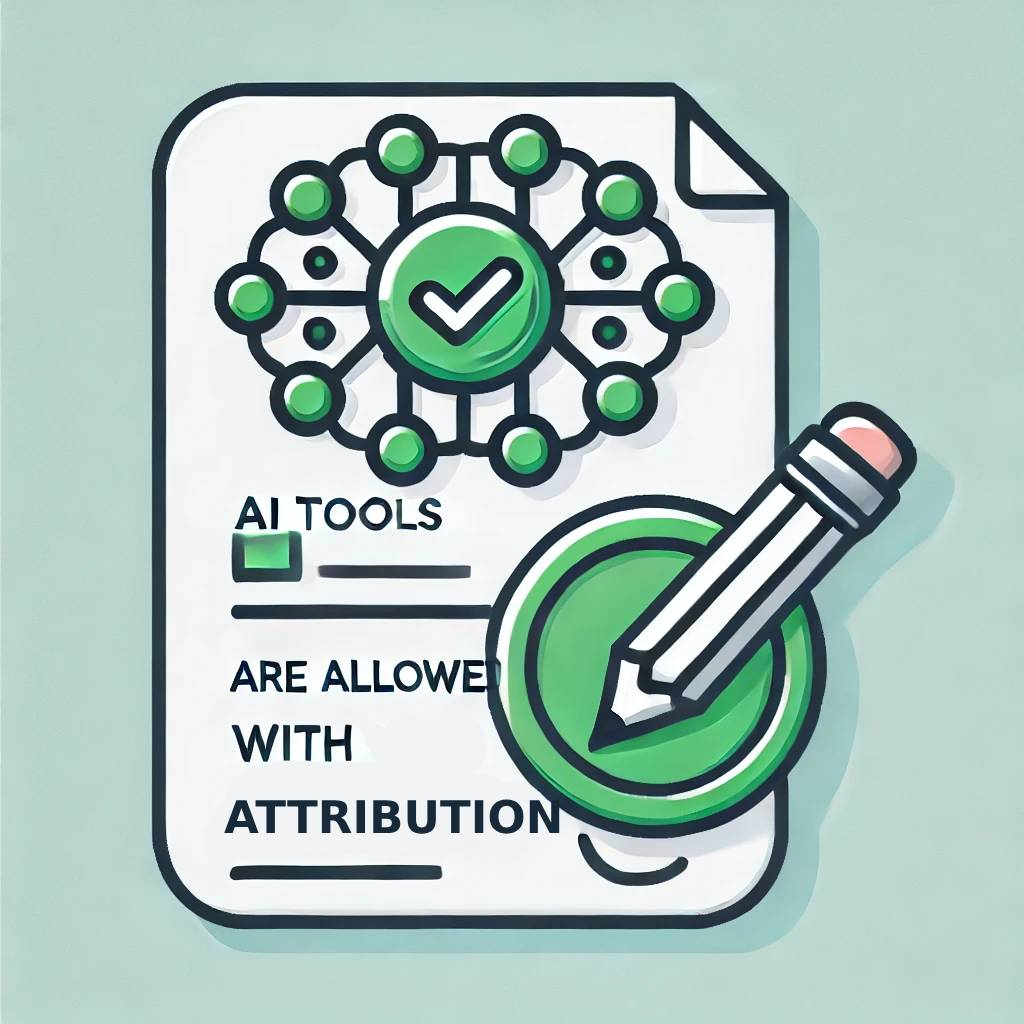
\includegraphics[width=1cm]{figs/Allowed_with_contributino.jpg}
     فرض کنید $f: \mathbb{R}^n \to \mathbb{R}$ یک تابع مشتق‌پذیر پیوسته به فرم زیر است:

    \[
    f(x) = \exp(-\|Ax - b\|^2) + \sin\left(\sum_{i=1}^{n} c_i x_i^2\right)
    \]
    
    که:
    \begin{itemize}
        \item $A \in \mathbb{R}^{n \times n}$ یک ماتریس با مرتبه کامل است.
        \item $b \in \mathbb{R}^n$ یک بردار بایاس است.
        \item $c_i \in \mathbb{R}$ ضرایب ثابت نامنفی یا صفر هستند.
    \end{itemize}
    
    ثابت کنید که برای هر مقدار $\epsilon > 0$ حداقل یک شبکه پرسپترون چند لایه $F(x)$ با تعداد محدودی نورون وجود دارد که بتواند تابع $f(x)$ را به‌طور دلخواه در یک دامنه فشرده $D \subset \mathbb{R}^n$ تقریب بزند به‌طوری‌که:(15 نمره)
    
    \[
    \| f(x) - F(x) \|_{L_2} < \epsilon
    \]
    
    \textbf{راهنما:} برای حل این مسئله ابتدا تابع $f(x)$ را به دو بخش نمایی و سینوسی تقسیم کنید. سپس با استفاده از مبانی تئوری و شبکه‌های عصبی چندلایه، هر بخش را به‌طور جداگانه تقریب بزنید. می‌توانید از منابع زیر برای اثبات خود کمک بگیرید:

    \lr{
    \begin{itemize}
        \item \href{https://cognitivemedium.com/magic_paper/assets/Hornik.pdf}{\lr{Multilayer Feedforward Networks are Universal Approximators}}
        \item \href{https://hal.science/hal-03753170/file/Cybenko1989.pdf}{\lr{Approximation by superpositions of a sigmoidal function}}
    \end{itemize}
    }

    \item 
\includegraphics[width=1cm]{figs/Forbidden_AI.jpg}
   اثبات کنید که افزودن یک ترم \( L_2 \) به تابع هزینه:
    \[
    R_\lambda (F) = R(F) + \lambda \| W \|_2^2
    \]
    واریانس مدل را کاهش داده و به بهبود تعمیم‌دهی کمک می‌کند. تأثیر پارامتر \( \lambda \) بر کران تعمیم (\lr{generalization bound}) را استخراج کنید(10 نمره).


    \item 
\includegraphics[width=1cm]{figs/Forbidden_AI.jpg}
    تصور کنید چند سال از فارغ‌التحصیلی شما گذشته و حالا در یک شرکت مشغول به کار هستید. به این نتیجه رسیده‌اید که به‌جای صعود در مسیر شغلی دیگران، کسب‌وکار شخصی خود را راه‌اندازی کنید. شما یک وب‌سایت آموزشی مفید و الهام‌بخش ساخته‌اید که حالا بازدیدکنندگان زیادی دارد و می‌خواهید از طریق تبلیغات آنلاین درآمد کسب کنید(15 نمره).

    برای کسب حداکثر درآمد از تبلیغات، به‌جای نمایش تصادفی تبلیغات، از یک سیستم حراجی استفاده می‌کنید که بهترین تبلیغات را برای هر موقعیت انتخاب می‌کند. اطلاعات تبلیغات در جدولی ثبت می‌شود که شامل موارد زیر است:
    
    \begin{itemize}
        \item \textbf{\lr{adv\_id}:} شناسه تبلیغ‌دهنده
        \item \textbf{\lr{cam\_id}:} شناسه کمپین تبلیغاتی
        \item \textbf{\lr{bid}:} مبلغ پیشنهادی برای هر کلیک یا اقدام
        \item \textbf{\lr{type}:} نوع درآمد (کلیک یا اقدام خاص)
        \item \textbf{\lr{pos\_id}:} موقعیت تبلیغ در سایت
        \item \textbf{\lr{ad\_id}:} شناسه تبلیغ
        \item \textbf{\lr{views}:} تعداد نمایش تبلیغ
        \item \textbf{\lr{clicks}:} تعداد کلیک‌ها روی تبلیغ
        \item \textbf{\lr{actions}:} تعداد اقدامات انجام‌شده پس از کلیک
        \item \textbf{\lr{week\_id}:} زمان جمع‌آوری داده‌ها (بر اساس هفته)
    \end{itemize}
    
    \begin{table}[h!]
        \centering
        \begin{tabular}{|c|c|c|c|c|c|c|c|c|c|}
            \hline
            \textbf{\lr{adv id}} & \textbf{\lr{cam id}} & \textbf{\lr{bid}} & \textbf{\lr{type}} & \textbf{\lr{pos id}} & \textbf{\lr{ad id}} & \textbf{\lr{views}} & \textbf{\lr{clicks}} & \textbf{\lr{actions}} & \textbf{\lr{week id}} \\
            \hline
            1234 & 6575 & 1000 & \lr{Click}  & 10 & 8975 & 15436 & 15 & 0 & 1735115563 \\
            1234 & 6575 & 1000 & \lr{Click}  & 13 & 6735 & 18466 & 10 & 0 & 1735115563 \\
            4321 & 9876 & 9000 & \lr{Action} & 78 & 7185 & 10321 & 20 & 2 & 1735124569 \\
            5678 & 4532 &  500 & \lr{Click}  &  5 & 1024 & 21000 & 25 & 0 & 1735114563 \\
            2345 & 3456 & 2000 & \lr{Click}  & 20 & 2341 & 18000 & 30 & 0 & 1735118563 \\
            7890 & 7654 & 8000 & \lr{Action} & 25 & 6523 & 12000 & 18 & 5 & 1735134563 \\
            \hline
        \end{tabular}
    \end{table}
    ﺑﺎ ﺍﺳﺘﻔﺎﺩﻩ ﺍﺯ ﺍﯾﻦ ﺩﺍده ﻫﺎ ﻭ ﻓﺮﻣﻮﻝﻫﺎﯼ ﺑﻬﯿنه ﺳﺎﺯﯼ ﮐﻪ ﺩﺭ ﺍﺩﺍﻣﻪ ﺍﺭﺍﺋﻪ ﺷﺪﻩ ﺍﺳﺖ، می‌توانید ﺍﻧﺘﺨﺎﺏ ﺗﺒﻠﯿﻐﺎﺕ ﺭﺍ ﺩﺭ ﺟﺎیگاه ﻫﺎﯼ ﻣﺨﺘﻠﻒ ﺑﻬﯿﻨﻪ ﮐﻨﯿﺪ ﺗﺎ ﺩﺭﺁﻣﺪ ﺷﻤﺎ ﺣﺪﺍﮐﺜﺮ ﺷﻮﺩ. ﺑﻪ ﺍﯾﻦ ﺭﻭﺍﺑﻂ ﺩﻗﺖ ﮐﻨﯿﺪ ﻭ سعیﮐﻨﯿﺪ ﺩﺭﮎ ﮐﻨﯿﺪ که ﭼﺮﺍ ﺍﯾﻦ ﻓﺮﻣﻮﻝ ﻫﺎ می ﺗﻮﺍﻧﻨﺪ ﺑﻪ ﺍﻧﺘﺨﺎﺏ ﺗﺒﻠﯿﻐﺎﺗ ﺑﺎ ﺑﯿﺸﺘﺮﯾﻦ ﺩﺭﺁﻣﺪ ﻣﻮﺭﺩ ﺍﻧﺘﻈﺎﺭﮐمک ﮐﻨﻨﺪ.
    
    \textbf{فرمول بهینه‌سازی تبلیغات کلیکی}
    \[
    \text{\lr{For each position}} (p), \text{ :\lr{select}} \arg\max_{ad \in A(p)} (bid_{ad} \times ctr(ad, p))
    \]
    
    \textbf{فرمول بهینه‌سازی تبلیغات اکشنی}
    \[
    \text{\lr{For each position}} (p), \text{ :$select$ } \arg\max_{ad \in A(p)} (bid_{ad} \times ctr(ad, p) \times cvr_{ad})
    \]
    
    \begin{itemize}
        \item \( A(p) \): مجموعه تبلیغاتی که امکان نمایش در جایگاه \( p \) دارند.
        \item \( bid_{ad} \): مبلغی که تبلیغ‌دهنده برای هر کلیک پرداخت می‌کند.
        \item \( ctr(ad, p) \): احتمال کلیک کاربر بر روی تبلیغ \( ad \) در جایگاه \( p \) (نرخ کلیک).
        \item \( cvr_{ad} \): احتمال انجام اکشن توسط کاربر پس از کلیک روی تبلیغ.
    \end{itemize}
    
    فرض کنید مدل‌های آموزش داده شده در مواجهه با ورودی‌های ناشناخته (مانند تبلیغات، کمپین‌ها یا تبلیغ‌دهندگان جدید)، به‌صورت میانگین‌گیری سیستمایتک عمل می‌کنند. به طور مشخص، اگر یک تبلیغ جدید باشد اما کمپین مرتبط با آن قبلاً در سیستم دیده شده باشد، \( CTR \) و \( CVR \) آن تبلیغ به‌صورت میانگین وزنی از مقادیر مربوط به تبلیغات قبلی آن کمپین محاسبه می‌شود.
    
    \textbf{الف)}
    یکی از مهم‌ترین مراحل در فرآیند آموزش هر مدل یادگیری ماشین، تقسیم‌بندی داده‌ها به مجموعه‌های \lr{Train}، \lr{Dev}، \lr{Train-Dev} و \lr{Test} است. این کار به ما کمک می‌کند تا عملکرد مدل را بر روی توزیع داده‌های مختلف بررسی کنیم. در این مسئله خاص چطور این‌کار را باید انجام داد و در انتخاب این مجموعه‌ها به چه نکاتی باید توجه داشت؟
    
    \textbf{ب-۱)}
    در هر یک از سناریوهای زیر، به طور مختصر مشکل را معرفی کرده و راه‌حلی برای آن ارائه دهید:
    \begin{enumerate}
        \item از قطعیت داده‌های ورودی اطمینان داریم ولی خطای آموزش مدل (\lr{Training Error}) بالا است.
        \item خطای آموزش مدل پایین است ولی خطای آن روی مجموعه (\lr{Train-Dev}) همچنان بالا است.
        \item خطای مدل در مجموعه‌های \lr{Train} و \lr{Train-Dev} پایین است ولی روی مجموعه \lr{Dev} خطا زیاد است.
        \item خطای \lr{Dev} پایین است ولی روی مجموعه \lr{Test} خطا همچنان زیاد است.
    \end{enumerate}
    
    \textbf{ب-۲)}
    آیا در اولین سناریوی مطرح‌شده در قسمت قبل، افزایش سایز داده‌های آموزش راه‌حل خوبی خواهد بود؟
    
    \textbf{ب-۳)}
    فرض کنید مدل‌هایی که برای پیش‌بینی نرخ کلیک (\lr{CTR}) و نرخ تبدیل (\lr{CVR}) تبلیغات آموزش داده‌اید، در داده‌های آموزش به دقت بالایی دست یافته‌اند. با این حال، زمانی که این مدل‌ها بر روی داده‌های \lr{Dev} اعمال می‌شوند و شما قصد دارید درآمد را بهینه کنید، اختلاف قابل‌توجهی بین پیش‌بینی‌های مدل و درآمد واقعی مشاهده می‌کنید. علت این خطا را شناسایی کرده و تحلیل کنید که چه عواملی ممکن است باعث این اختلاف شوند.
    
    توجه: جدول ارائه شده صرفاً برای آشنایی با ساختار داده‌ها و فضای مسئله است و مقادیر آن فاقد اهمیت هستند.
    
    \textbf{ج)}
    در یک سیستم بهینه‌سازی تبلیغات مبتنی بر داده‌های واقعی، یکی از چالش‌های اساسی، مواجهه با تغییرات ناگهانی در رفتار کاربران (\lr{Concept Drift}) و نامتوازن بودن داده‌ها است. فرض کنید در دوره‌های زمانی خاصی (مانند مناسبت‌های خاص یا تغییر الگوریتم جستجو در موتورهای جستجو)، نرخ کلیک (\lr{CTR}) و نرخ تبدیل (\lr{CVR}) به‌طور ناگهانی دچار تغییرات چشمگیر می‌شوند.
    
    \begin{itemize}
        \item چگونه می‌توان پایداری مدل را در مواجهه با \lr{Concept Drift} تضمین کرد؟
        \item چه روش‌هایی برای مدیریت داده‌های نامتوازن در این مسئله مناسب هستند؟
        \item تحقیق کنید که چگونه می‌توان با استفاده از الگوریتم‌های آنلاین یادگیری (\lr{Online Learning})، عملکرد سیستم را بهبود بخشید و به تغییرات سریع بازار واکنش نشان داد.
    \end{itemize}
       
    \section*{سوالات عملی} 
    \item 
\includegraphics[width=1cm]{figs/Allowed_recommended.jpg}
    ($HousingData$) هدف این تمرین، پیش پردازش داده و پیاده سازی دستی ماژول های شبکه عصبی است. شما باید بخش‌های $\#TODO$ را تکمیل کنید. لذا از هرگونه تغییر یا دستکاری ساختار اصلی کد اجتناب فرمایید.کلیه کدها باید از قبل اجرا شده باشند؛ در غیر این صورت نمره مربوطه تعلق نخواهد گرفت(25 نمره).
    
    \item 
\includegraphics[width=1cm]{figs/Allowed_recommended.jpg}
    ($FashionMNIST$) هدف این تمرین، ایجاد ماژول های شبکه عصبی و ترکیب آنها جهت ساخت یک شبکه کامل است. شما باید بخش‌های $\#TODO$ و سوالاتی که در نوت‌بوک بیان شده را تکمیل کنید. لذا از هرگونه تغییر یا دستکاری ساختار اصلی کد اجتناب فرمایید. کلیه کدها باید از قبل اجرا شده باشند؛ در غیر این صورت نمره مربوطه تعلق نخواهد گرفت(35 نمره).
\end{enumerate}



\end{document}


